\documentclass[12pt]{report}
\usepackage{../header}

\renewcommand{\div}{\mathrm{div~}}
\newcommand{\grad}{\mathrm{grad~}}
\newcommand{\rot}{\mathrm{rot~}}

\DeclareDocumentCommand{\pp}{G{}m}{\frac{\partial{#1}}{\partial{#2}}}

\title{Тема 3. Бисферические, тороидальные, инверсные сферические, и иные ортогональные системы координат.}

\begin{document}
	\maketitle
	
Эту тему мы изучаем с целью упрощения решения уравнения Пуассона $\Delta\phi = -\rho/\epsilon_0$, возникающего в электростатике -- задача поиска распределения потенциала и, соответственно, поля, в резонаторе.

\paragraph{Оператор набла} $\nabla = (\frac{\partial}{\partial x}, \frac{\partial}{\partial y}, \frac{\partial}{\partial z})$.
\begin{itemize}
	\item $\nabla f \equiv \grad f = \vec g$ (градиент)
	\item $\nabla\cdot\vec g \equiv \div\vec g = f_1$ (дивергенция)
	\item $\nabla\times\vec g \equiv \rot\vec g = \vec g_1$ (ротор)
\end{itemize}

\paragraph{Оператор Лапласа}
Возьмём одно из уравнений Максвелла для электрического поля:
\[
\div \vec E = \rho/\epsilon_0,
\]
и представим $\vec E = -\grad \phi$, где $\phi$ -- потенциал.

Тогда
\[
\div\grad\phi \equiv \nabla^2 \phi \equiv \Delta\phi = \rho/\epsilon_0.
\]

$\Delta$ называется \emph{оператором Лапласа}:
\[
\nabla^2 = \nabla\cdot\nabla = \frac{\partial^2}{\partial x^2} + \frac{\partial^2}{\partial y^2} + \frac{\partial^2}{\partial z^2}.
\]


\section{Ортогональные криволинейные координаты}
\begin{figure}[h!]\centering
	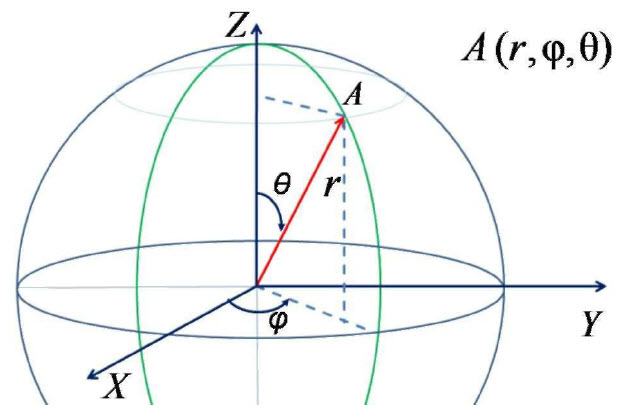
\includegraphics[width=\linewidth]{spherical_cs}
	\caption{Сферическая система координат.\label{fig:spherical_cs}}
\end{figure}

Любые три параметра $(q_1,q_2,q_3)$, однозначно определяющие положение точки в пространстве, могут быть выбраны в качестве координат этой точки. Такие координаты называются \emph{независимыми обобщёнными координатами}.~\cite[стр.~5]{Alferov} Например, на Рисунке~\ref{fig:spherical_cs} изображена сферическая система координат, в которой положение задаётся двумя углами и длиной радиус-вектора. 

Сферические координаты связаны с Декартовыми формулами:
\begin{equation}\label{eq:spherical-to-cartesian}
	\begin{cases}
	x &= r\sin\Theta\cos\phi, \\
	y &= r\sin\Theta\sin\phi, \\
	z &= r\cos\Theta.
	\end{cases}
\end{equation}

В общем виде, уравнение~\eqref{eq:spherical-to-cartesian} можно записать как
\begin{equation}\label{eq:general-cs-to-cartesian}
	\begin{cases}
		x &= x(q_1,q_2,q_3), \\
		y &= y(q_1, q_2, q_3), \\
		z &= z(q_1, q_2, q_3).
	\end{cases}
\end{equation}
Решая систему уравнений~\eqref{eq:general-cs-to-cartesian} можно найти обратные соотношения, выражающие криволинейные точки в функции от декартовых координат.~\cite[стр.~5]{Alferov} 

 \section{Коэффициенты Ламэ}
Запишем бесконечно малый вектор $\rd\vec s$ в декартовых и обобщённых координатах:
\begin{subequations}
	\begin{equation}\label{eq:ds-in-cartesian}
		\rd\vec s = \vec i \rd x+ \vec j\rd y + \vec k\rd z,
	\end{equation}
	\begin{equation}\label{eq:ds-in-generic}
		\rd\vec s = \vec e_1\rd q_1 + \vec e_2\rd q_2+ \vec e_3\rd q_3.
	\end{equation}
\end{subequations}
Записав полные дифференциалы функций~\eqref{eq:general-cs-to-cartesian}, и приравняв правые части~\eqref{eq:ds-in-cartesian} и~\eqref{eq:ds-in-generic}, получим:
\begin{equation*}
	\vec e_\alpha = \vec i\pp{x}{q_\alpha} + \vec j \pp{y}{q_\alpha} + \vec k\pp{z}{q_\alpha},~\alpha\in\{1,2,3\}.
\end{equation*}

Норма $||\vec e_i|| = \vec e_i\cdot\vec e_i$ называется \emph{коэффициентом Ламэ} $H_i$ для координаты $q_i$ в точке $M$:
\begin{equation}\label{eq:Lame-1}
H_i = \sqrt{\left(\pp{x}{q_i}\right)^2 + \left(\pp{y}{q_i}\right)^2 + \left(\pp{z}{q_i}\right)^2}.
\end{equation}

\paragraph{Дифференциал  длины дуги}
%[КАРТИНКА!!!]
Запишем длину дуги кривой:
\begin{equation*}
	\rd r^2 = \rd\vec r\cdot\rd\vec r = ||\vec e_1||\rd q_1^2 + ||\vec e_2||\rd q_2^2 + ||\vec e_3||\rd q_3^2.
\end{equation*}

Отсюда следует, что коэффициент Ламе можно выразить как частную производную длины дуги по соответствующей обобщённой координате:
\begin{equation}\label{eq:Lame-2}
	H_i = \left|\pp{\vec r}{q_i}\right|.
\end{equation}
 Ожидаемо, выражение получается то же, что и в~\eqref{eq:Lame-1}.

\paragraph{Элемент объёма}
%[КАРТИНКА!!!]
\begin{align}
	\rd V &= \rd x\rd y\rd z \notag\\
	&= \det J \cdot \rd q_1\rd q_2\rd q_3 \notag\\
	&= H_1H_2H_3\cdot \rd q_1\rd q_2\rd q_3. \label{eq:unit-volume}
\end{align}
Здесь 
\[
J = \left[\begin{matrix}
\pp{x}{q_1} & \pp{x}{q_2} & \pp{x}{q_3} \\
\pp{y}{q_1} & \pp{y}{q_2} & \pp{y}{q_3} \\
\pp{z}{q_2} & \pp{z}{q_2} & \pp{z}{q_3}
\end{matrix}\right]
\]
якобиан.~\cite{Jacobian}

\paragraph{Лапласиан}
\newcommand{\HHH}[3]{\frac{H_{#1}H_{#2}}{H_{#3}}}
\begin{align}
	\Delta f(q_1,q_2,q_3) = \frac{1}{H_1 H_2 H_3}
	\left[
	      \pp{}{q_1}\left(\HHH{2}{3}{1}\pp{f}{q_1}\right) 
	+ \pp{}{q_2}\left(\HHH{1}{3}{2}\pp{f}{q_2}\right)\right. \notag\\
	+ \left.\pp{}{q_3}\left(\HHH{1}{2}{3}\pp{f}{q_3}\right)
	\right] \label{eq:Laplacian}
\end{align}

 \section{Различные системы координат}
 Выражения для коэффициентов Ламэ и Лапласиана легко гуглятся; в крайнем случае, пользуемся уравнениями~\eqref{eq:Lame-1} и~\eqref{eq:Laplacian}. Я громоздкие формулы спрашивать не буду. 
 Поэтому акцент сделаем на генеологии систем координат.
 
 В принципе, у нас любая криволинейная система координат задаётся семействами кривых, которые пересекаются под прямыми углами в каждой точке. 
 \subsection{Эллиптическая $\to$ эллипсоидальная}
\begin{figure}[h]\centering
 	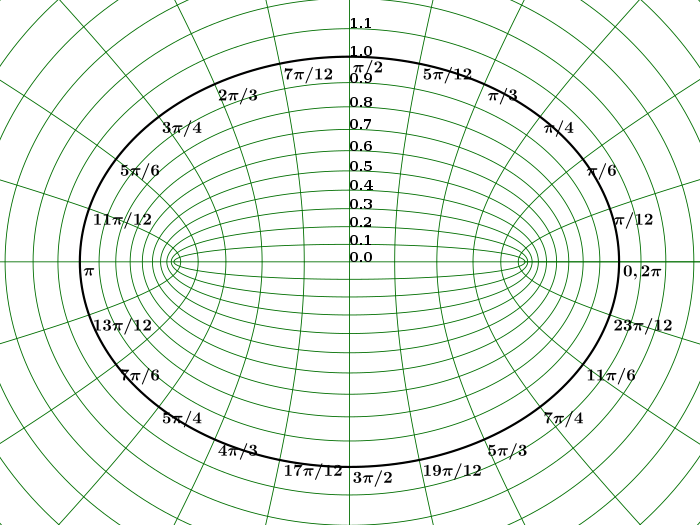
\includegraphics[width=.8\linewidth]{elliptical_coordinates}
 	\caption{Эллиптическая система координат состоит из софокусных эллипсов и гиперболоидов.}
\end{figure}
\begin{figure}[h]\centering
 	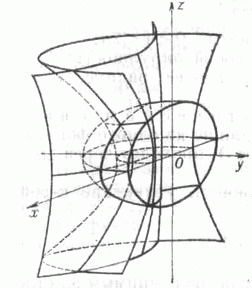
\includegraphics[height=.35\paperheight]{ellipsoidal_cs}
 	\caption{Эллипсоидальная система: эллипсоид + одно- и двуполостные эллипсоиды.}
\end{figure}

 \subsection{Биполярная и бисферическая}
 \begin{figure}[h]\centering
 	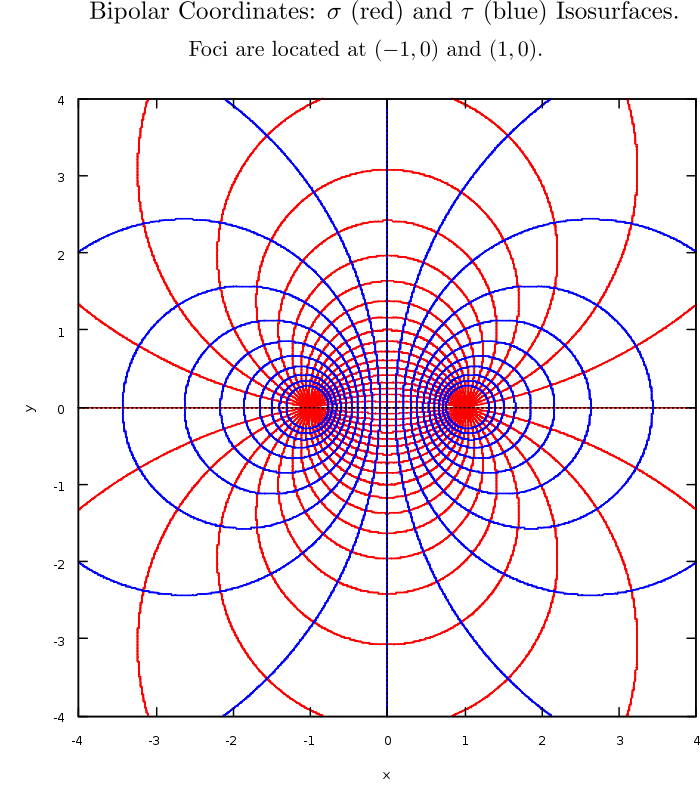
\includegraphics[width=.8\linewidth]{bipolar_cs}
 	\caption{Биполярная КС состоит из кругов Апполония.}
 \end{figure}
\begin{figure}[h]\centering
	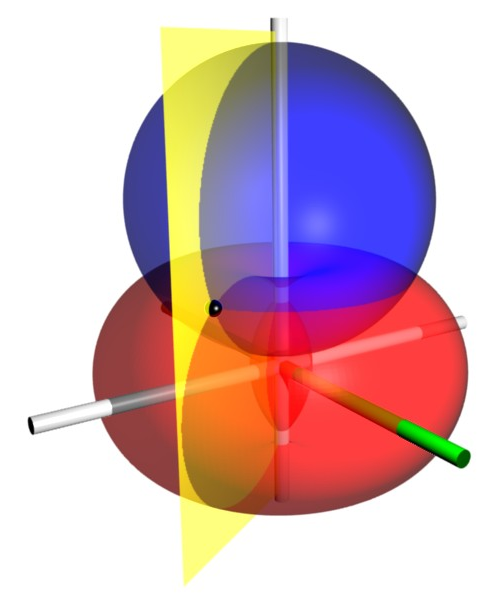
\includegraphics[height=.33\paperheight]{Bispherical_coordinates}
	\caption{Бисферическая КС -- тело вращения биполярной КС вокруг оси, \emph{проходящей через} фокусы.}
\end{figure}
 
 \subsection{Тороидальная КС}
\begin{figure}[h]\centering
	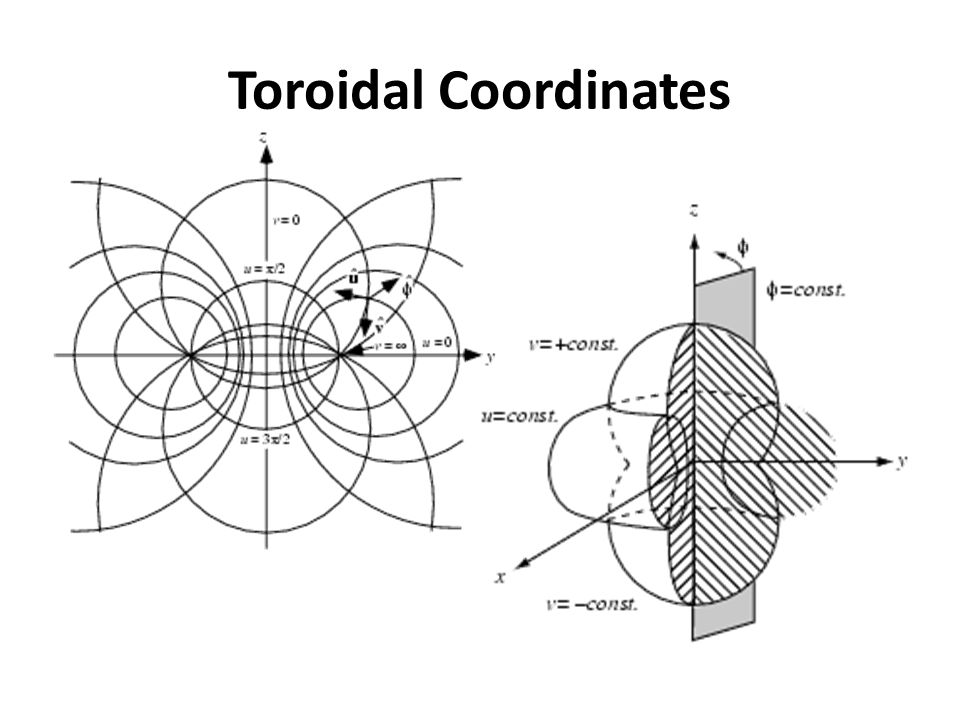
\includegraphics[width=\linewidth]{toroidal_cs}
	\caption{Получается из биполярной при вращении последней вокруг оси, \emph{разделяющей} фокусы.}
\end{figure}

\section{Задачи}
\paragraph{\#1}
\emph{Вывести формулы преобразования от эллипсоиидальных координат к декартовым.}

Эллипсоидальная СК задаётся эллипсоидом и двумя гиперболоидами (одно- и двух-полостным)~\cite{Ellipsoidal-cs},
т.е. системой уравнений
\begin{equation*}
\begin{cases}
	\frac{x^2}{a^2 + \xi} + \frac{y^2}{b^2 + \xi} + \frac{z^2}{c^2 + \xi} &= 1,\\
	\frac{x^2}{a^2 + \eta} + \frac{y^2}{b^2 + \eta} + \frac{z^2}{c^2 + \eta} &= 1,\\
	\frac{x^2}{a^2 + \zeta} + \frac{y^2}{b^2 + \zeta} + \frac{z^2}{c^2 + \zeta} &= 1,
\end{cases}
\end{equation*}
где $-c^2 < \xi < \infty$, $-b^2 < \eta < -c^2$, $-a^2 < \zeta < -b^2$.

Разрешая систему относительно $x^2,y^2mz^2$ получаем что надо.

\begin{thebibliography}{0}
	\bibitem{Alferov}
	Г.В. Алферов. Механика в криволинейных координатах. Пособие для подготовки к коллоквиуму.
	\url{http://www.apmath.spbu.ru/ru/staff/alferov/files/krivol_coordinaty.pdf}
	\bibitem{Lame-coef}
	В.В. Конев. Скалярные и векторные поля.
	\url{http://portal.tpu.ru:7777/SHARED/k/KONVAL/Sites/Russian_sites/T_field/manual/38.htm}
	\bibitem{Jacobian}
	Wolfram. Jacobian.
	\url{http://mathworld.wolfram.com/Jacobian.html}
	\bibitem{Ellipsoidal-cs}
	Wolfram. Confocal Ellipsoidal Coordinates.
	\url{http://mathworld.wolfram.com/ConfocalEllipsoidalCoordinates.html}
\end{thebibliography}

\end{document}